\section{Experiments and Mechanistic Analysis}
\label{sec:experiments}

We conduct a causal audit across seven experimental modules (\texttt{Pilot}, \texttt{E1}, \texttt{E2-A}, \texttt{E3-A/B/C}, \texttt{E5}, \texttt{E6}, and \texttt{E7}), totaling over $200,000$ forward and intervention passes. All bracketed confidence intervals represent $5,000$-iteration scene-cluster bootstrap $95\%$ intervals, averaging templates and edits within each source scene cluster before resampling.

\subsection{Destructive Slot Interference Across $K \in \{1, 2, 4\}$ (\texttt{Pilot}, \texttt{E1}, \texttt{E3-C}, \texttt{E7-2})}
\label{subsec:exp_e3c}

\textbf{Single-Hop Public Benchmarks (\texttt{Pilot}).} Across $991$ public single-hop examples in TreeBench~\cite{treebench2025} ($400$), HR-Bench 4K/8K~\cite{wang2024hrbench} ($400$), and V*Bench~\cite{wu2024vstar} ($191$), native \texttt{LVR-7B} ($L \in \{4, 8, 16\}$) achieves $48.51\%$--$48.81\%$ weighted accuracy, matching \texttt{NoLatent} ($48.76\%$), slot zeroing ($H \leftarrow 0$, $48.81\%$), and Gaussian noise ($48.56\%$), whereas decoding-time \texttt{Vision-Mask} drops accuracy to $28.61\%$ (Supplementary Table~S1), consistent with single-hop non-portability~\cite{guo2026beyond}.

\begin{table*}[!t]
  \caption{\textbf{Same-Scene Single- and Multi-Step Component Dissociation on 150 Frozen Scene Clusters (\texttt{E3-C} $9,600$ Runs \& \texttt{E7-2} $13,200$ Outputs).} Left: $K=1$ single-hop accuracy on Template 0 ($600$ queries/arm, \texttt{E7-2}). Middle \& Right: $K \in \{2, 4\}$ full-chain exact-match accuracy ($\%$) and $K=4$ per-position mean ($\%$) / slope (pp/step) across both templates (\texttt{E3-C}). Boundary markers (\texttt{Marker-only}) are neutral ($\pm 0.67$pp), whereas native non-zero slots induce $-16.00$ to $-21.67$pp single-hop and $-10.33$ to $-20.00$pp multi-step degradation, $100\%$ recovered by \texttt{Zero-Slot}.}
  \label{tab:e3c}
  \centering
  \resizebox{\textwidth}{!}{%
  \begin{tabular}{l c c c c c c c}
    \toprule
    & \textbf{$K=1$ Single-Hop} & \multicolumn{4}{c}{\textbf{Multi-Step Full-Chain Exact-Match Accuracy (\texttt{E3-C}, \%)}} & \multicolumn{2}{c}{\textbf{$K=4$ Position Mean (\%) / Slope}} \\
    \cmidrule(lr){2-2} \cmidrule(lr){3-6} \cmidrule(lr){7-8}
    \textbf{Strategy / Intervention Arm} & \textbf{(\texttt{E7-2} T0, \%)} & \textbf{$K=2$ Indep.} & \textbf{$K=2$ Serial} & \textbf{$K=4$ Indep.} & \textbf{$K=4$ Serial} & \textbf{$K=4$ Indep.} & \textbf{$K=4$ Serial} \\
    \midrule
    \texttt{NoLatent} & $83.33\ci{80.50}{86.17}$ & $76.00\ci{70.00}{82.33}$ & $\mathbf{73.67}\ci{66.67}{80.33}$ & $30.67\ci{24.00}{37.67}$ & $35.00\ci{27.67}{42.00}$ & $68.67 / {-6.53}$ & $71.50 / {-5.33}$ \\
    \texttt{Marker-only} ($L=0$) & $83.50\ci{80.50}{86.33}$ & $76.33\ci{70.00}{82.33}$ & $73.33\ci{66.66}{79.67}$ & $31.33\ci{24.33}{38.33}$ & $34.33\ci{27.00}{41.67}$ & $68.58 / {-6.03}$ & $70.42 / {-4.77}$ \\
    \texttt{Native} $L=4$ ($L=2$: $67.33\%$ on $K{=}1$) & $63.33\ci{58.83}{67.67}$ & $64.00\ci{57.00}{70.67}$ & $63.00\ci{56.33}{69.67}$ & $18.00\ci{13.00}{23.33}$ & $21.00\ci{15.33}{27.00}$ & $58.58 / {-3.83}$ & $61.33 / {-2.07}$ \\
    \texttt{Native} $L=8$ & $61.67\ci{57.33}{66.00}$ & $56.33\ci{49.00}{63.34}$ & $57.00\ci{49.67}{64.00}$ & $19.00\ci{13.67}{24.33}$ & $24.33\ci{18.67}{30.33}$ & $61.00 / {-2.80}$ & $63.92 / {-1.10}$ \\
    \rowcolor{resulttint}
    \texttt{Zero-Slot} $L=4$ & $\mathbf{83.67}\ci{80.83}{86.50}$ & $\mathbf{77.00}\ci{71.00}{83.00}$ & $73.33\ci{66.33}{79.67}$ & $32.67\ci{25.67}{39.67}$ & $\mathbf{36.33}\ci{29.33}{43.67}$ & $\mathbf{68.83} / {-7.00}$ & $\mathbf{72.08} / {-5.77}$ \\
    \rowcolor{resulttint}
    \texttt{Zero-Slot} $L=8$ & $\mathbf{83.67}\ci{80.83}{86.33}$ & $76.33\ci{70.00}{82.33}$ & $72.33\ci{65.67}{79.00}$ & $\mathbf{33.33}\ci{26.33}{40.33}$ & $\mathbf{36.33}\ci{29.00}{43.67}$ & $68.67 / {-7.53}$ & $72.00 / {-6.93}$ \\
    \texttt{Zero-Marker} $L=4$ & $62.83\ci{58.33}{67.33}$ & $64.33\ci{57.33}{71.33}$ & $62.67\ci{55.67}{69.33}$ & $19.00\ci{14.00}{24.00}$ & $21.00\ci{15.67}{26.67}$ & $59.00 / {-3.87}$ & $61.83 / {-2.27}$ \\
    \texttt{Zero-Marker} $L=8$ & $61.83\ci{57.50}{66.17}$ & $56.33\ci{49.33}{63.33}$ & $57.00\ci{50.00}{64.00}$ & $19.67\ci{14.33}{25.00}$ & $25.33\ci{19.33}{31.67}$ & $61.92 / {-3.37}$ & $65.00 / {-0.73}$ \\
    \midrule
    \texttt{Marker-only} $-$ \texttt{NoLatent} & $+0.17\ci{-0.50}{1.00}$ & $+0.33\ci{0.00}{1.00}$ & $-0.33\ci{-2.00}{1.33}$ & $+0.67\ci{-0.67}{2.00}$ & $-0.67\ci{-2.00}{0.67}$ & \multicolumn{2}{c}{Markers neutral; \texttt{Zero-Slot} $L{=}8{-}\text{Nat}{=}+12.0\text{--}22.0$pp} \\
    \texttt{Zero-Slot} $-$ \texttt{Native} ($L=4$) & $\mathbf{+20.33}\ci{16.17}{24.83}$ & $\mathbf{+13.00}\ci{6.67}{19.33}$ & $\mathbf{+10.33}\ci{4.00}{16.67}$ & $\mathbf{+14.67}\ci{8.67}{20.67}$ & $\mathbf{+15.33}\ci{10.00}{20.67}$ & \multicolumn{2}{c}{$100\%$ recovery via slot zeroing} \\
    \bottomrule
  \end{tabular}%
  }
\end{table*}

\begin{figure}[!t]
  \centering
  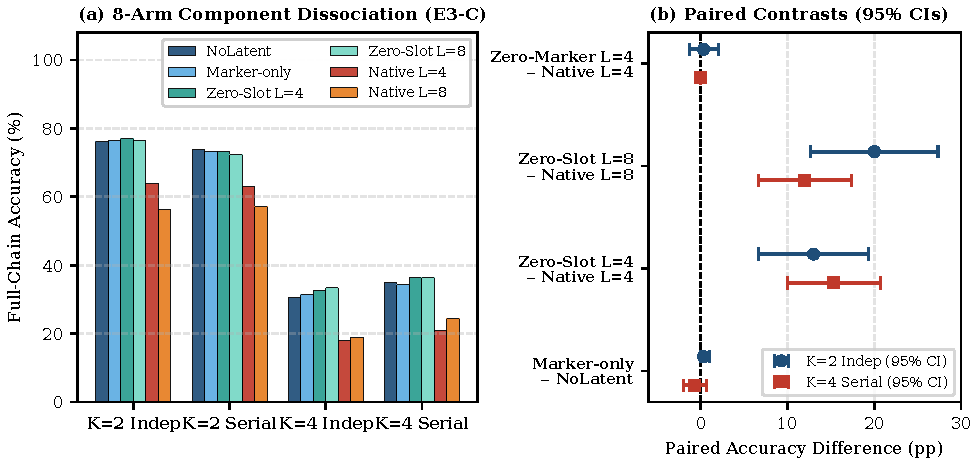
\includegraphics[width=\linewidth]{figs/fig2_e3c_slot_interference.pdf}
  \caption{\textbf{Destructive Slot Interference Across $K \in \{1, 2, 4\}$ (\texttt{E3-C} \& \texttt{E7-2}).} \textbf{(a)} Same-scene accuracy on 150 frozen clusters ($K=1$ on Template 0; $K=2, 4$ full-chain across both templates). \textbf{(b)} Paired cluster-bootstrap differences ($95\%$ CI, $L=4$): boundary markers are neutral ($\pm 0.67$pp), whereas \texttt{Zero-Slot} minus \texttt{Native} yields $+20.33$pp on $K=1$ and $+10.33$--$15.33$pp on $K=2, 4$ ($+20.00$pp at $L=8$).}
  \label{fig:e3c}
\end{figure}

\textbf{Same-Scene $K \in \{1, 2, 4\}$ Component Dissociation (\texttt{E1}, \texttt{E3-C}, \texttt{E7-2}).} Across the $150$ frozen clusters (\cref{tab:e3c}, \cref{fig:e3c}, and Supplementary Table~S14), native rollouts cause severe negative transfer across both single- and multi-step queries. On $K=2, 4$ (\texttt{E3-C}, $9,600$ runs), \texttt{NoLatent} $K=4$ independent and serial chain accuracies are $30.67\%$ and $35.00\%$ (serial position mean $\bar{p}=71.50\%$ exceeds $\bar{p}^4 = 26.13\%$ due to within-scene correlation $\mathrm{Cov}(C_j, C_k) > 0$, Proposition~\ref{prop:margin}; serial-vs-independent interaction $I_{\mathrm{fixed}} = -2.67\ci{-9.33}{4.00}$pp spans zero). Native rollouts ($L=4, 8$) lower per-position accuracy by $\pi_k^- - \pi_k^+ \approx 10.1$pp ($71.50\% \to 61.33\%$ on $K=4$ serial), compounding via Eq.~\eqref{eq:multistep_telescope} into a $10.33$--$20.00$pp full-chain drop ($35.00\% \to 21.00\%$ on $K=4$ serial; $76.00\% \to 56.33\%$ on $K=2$ indep.\ $L=8$).
Evaluating all $11$ arms ($L \in \{2, 4, 8\}$) on single-hop $K=1$ queries on the \emph{exact same 150 scenes} (\texttt{E7-2}, $13,200$ outputs) shows that \texttt{Native} $L=2/4/8$ already drops $K=1$ accuracy from $83.33\%$ (\texttt{NoLatent}) to $67.33\% / 63.33\% / 61.67\%$ ($\mathbf{-16.00}$\textbf{, }$\mathbf{-20.00}$\textbf{, and }$\mathbf{-21.67}$\textbf{pp}), whereas \texttt{Marker-only} ($83.50\%$) and \texttt{Zero-Slot} ($83.67\%$) restore $100\%$ of \texttt{NoLatent} accuracy. Thus, destructive slot interference is \emph{not} exclusive to multi-step tracking: by Proposition~\ref{prop:margin}, same-color distractors place baseline margins near $M_k=0$, exposing negative slot shifts $\Delta M_k^{\mathrm{slot}}(H) < 0$ even at $K=1$ ($K=1$ \texttt{NoLatent} $83.33\%$ is slightly below $K=2$ independent per-position $88.00\%$ on Template 0 due to prompt/length differences).

\subsection{Input Sensitivity vs.\ Zero Readout (\texttt{E2-A}, \texttt{E3-A/B})}
\label{subsec:exp_e3b}

\textbf{Input Sensitivity (\texttt{E2-A}) vs.\ Donor Swap (\texttt{E3-A}).} Across the $87$ counterfactual pairs ($3,192$ \texttt{E2-A} runs), recoloring the step-$m$ target ($\Vrel$) flips native \texttt{LVR-7B} predictions on $61.90\%$--$72.09\%$ of pairs ($0.00\%$ false flips on $\Virrel$) and shifts $H$ by $\|\Delta H\|_2 = 69.25$ (Supplementary Table~S2). Yet across $15,484$ \texttt{E3-A} runs ($384$ doubly eligible injections), patching $H(\Vrel)$ into $\Vorig$ yields \textbf{$0.00\%$} target flips (Supplementary Table~S3), while \texttt{Zero-Patch} on this pre-filtered $C_k^{(H)}=1$ subset retains the original answer on $95.35\%$--$98.86\%$ of instances, matching Proposition~\ref{prop:margin}.

\begin{table}[!t]
  \caption{\textbf{Local Visual Patch Swap Positive Control vs.\ ROI-Masked Latent Injection (\texttt{E3-B1}) and Logit Shift (\texttt{E3-B2}, $19,152$ Runs).} Target-step net directional transfer (pp) on Full / Position-Eligible / Chain-Eligible subsets, and full-set conditional log-odds shift $\delta M(1)$ (Unmasked / Vision-Masked).}
  \label{tab:e3b}
  \centering
  \resizebox{\linewidth}{!}{%
  \begin{tabular}{l c c c}
    \toprule
    \textbf{Cond.} & \textbf{Pos.\ Control: Visual Patch} & \textbf{ROI-Masked Latent} & \textbf{Logit Shift $\delta M(1)$} \\
    $(K, L)$ & \textbf{Swap (Full / Pos / Chain)} & \textbf{Swap (Full / Pos / Chain)} & \textbf{(Unmask / V-Mask)} \\
    \midrule
    $(2, 4)$  & $+48.8 / \mathbf{+83.9} / \mathbf{+85.4}$ & $-1.2 / \phantom{+}0.0 / +2.1$ & $-0.068 / {-0.070}$ \\
    $(2, 8)$  & $+50.0 / \mathbf{+87.0} / \mathbf{+91.3}$ & $-2.4 / \phantom{+}0.0 / \phantom{+}0.0$ & $-0.092 / {-0.072}$ \\
    $(2, 16)$ & $+53.7 / \mathbf{+93.5} / \mathbf{+93.8}$ & $-2.4 / \phantom{+}0.0 / \phantom{+}0.0$ & $-0.095 / {-0.060}$ \\
    $(4, 4)$  & $+42.7 / \mathbf{+87.6} / \mathbf{+89.8}$ & $+0.5 / +2.6 / \mathbf{\phantom{+}0.0}$ & $-0.016 / {-0.012}$ \\
    $(4, 8)$  & $+46.7 / \mathbf{+90.5} / \mathbf{+91.9}$ & $-0.7 / {-0.8} / \mathbf{\phantom{+}0.0}$ & $-0.015 / {-0.011}$ \\
    $(4, 16)$ & $+49.4 / \mathbf{+85.5} / \mathbf{+86.7}$ & $-0.8 / {-1.3} / \mathbf{\phantom{+}0.0}$ & $-0.026 / {-0.021}$ \\
    \bottomrule
  \end{tabular}%
  }
\end{table}

\textbf{Positive Control (\texttt{E3-B1}) and Logit Probing (\texttt{E3-B2}).} Across $19,152$ runs on the $266$ paired records (\cref{tab:e3b}), keeping $H(\Vorig)$ fixed and replacing only the visual tokens inside the target bounding box (\texttt{Visual Patch Swap}) flips \textbf{$83.93\%$--$93.75\%$} of eligible instances ($42.71\%$--$53.66\%$ full set). Conversely, masking those target-ROI visual keys during text decoding and injecting $H(\Vrel)$ yields near-zero net transfer ($-2.44$pp to $+2.56$pp), and 8-point interpolation $\alpha \in [0, 2]$ (\texttt{E3-B2}) yields flat/negative shifts across all $12$ conditions ($\delta M(1) \in [-0.0949, -0.0109]$; \cref{fig:logit_curves}).

\subsection{Decoding-Masked Adaptation and 28-Layer KV Double Dissociation (\texttt{E5} \& \texttt{E6-C})}
\label{subsec:exp_e5_e6c}

\textbf{Eliminating Interference Without Awakening Slots (\texttt{E5}).} Adapting \texttt{LVR-7B} on the $40$ dev training clusters ($2$ epochs, $160$ updates) with step-wise ROI alignment, $0.1\times$ 8-color CE, and $60\%$ decoding-time vision masking ($m_{\mathrm{vis}}=0$, $\mathrm{TBPTT}=1$) eliminates slot interference on the $150$ clusters ($K=4$ serial jumps by $\mathbf{+49.00}$\textbf{pp} to $70.00\%$; $K=4$ independent by $\mathbf{+51.67}$\textbf{pp} to $70.67\%$, matching adapted \texttt{NoLatent} at $70.00\%$), while \texttt{Vision-Masked} accuracy surges from ${\sim}3\%$ to \textbf{$82.33\%$--$85.33\%$} ($K=2$) and \textbf{$67.00\%$--$69.67\%$} ($K=4$; Supplementary Table~S7). Yet across $20,482$ post-adaptation \texttt{E3-A} runs, donor latent transfer under both unmasked and \texttt{Vision-Masked} decoding remains \textbf{$0.00\%\ci{0.00}{0.00}$} (Supplementary Table~S6).

\begin{table}[!t]
  \caption{\textbf{28-Layer KV-Cache Double Dissociation on the \texttt{E5} Checkpoint Under \texttt{Vision-Masked} Decoding (\texttt{E6-C}).} Target-position flip rates ($\%$) across $266$ counterfactual records. Swapping 28-layer latent caches ($\KV_H$, Arm C2) yields $0.00\%$ flips, whereas swapping prefill prompt/marker caches ($\KV_{Q,M}$, Arms C3a/b) yields $96.88\%$--$100.00\%$ flips on eligible subsets ($16.46\%$--$40.23\%$ full set). Blinding prefill caches (Arm C4) on the 150 clusters drops masked accuracy by $64.00$--$73.00$pp.}
  \label{tab:e6c}
  \centering
  \resizebox{\linewidth}{!}{%
  \begin{tabular}{l c c c c c}
    \toprule
    \textbf{Subset / Task} & \textbf{C1: Tape} & \textbf{C2: 28-L} & \textbf{C3a: Prompt} & \textbf{C3b: All Text} & \textbf{All-Vis.} \\
    (Records / Clusters) & $H$ \textbf{Swap} & $\KV_H$ \textbf{Swap} & $\KV_{Q,\mathrm{start}}$ & $\KV_{Q,\mathrm{mkr}}$ & \textbf{Donor Ref.} \\
    \midrule
    $K=2$ Full ($92/41$)    & $0.00$ & $0.00$ & $\mathbf{16.46}$ & $\mathbf{16.46}$ & $16.46$ \\
    \rowcolor{resulttint}
    $K=2$ Pos/Chn ($17/9$)  & $0.00$ & $0.00$ & $\mathbf{100.00}$ & $\mathbf{100.00}$ & $100.00$ \\
    $K=4$ Full ($174/64$)   & $0.00$ & $0.00$ & $\mathbf{40.23}$ & $39.19$ & $39.58$ \\
    \rowcolor{resulttint}
    $K=4$ Pos.\ ($73/32$)   & $0.00$ & $0.00$ & $\mathbf{96.88}$ & $\mathbf{96.88}$ & $100.00$ \\
    \rowcolor{resulttint}
    $K=4$ Chain ($63/27$)   & $0.00$ & $0.00$ & $\mathbf{100.00}$ & $\mathbf{100.00}$ & $100.00$ \\
    \midrule
    \multicolumn{6}{l}{\textbf{C4 Blind Prefill (150 Clust.):} $K{=}2$ S/I $\mathbf{-72.0 / {-73.0}\text{pp}}$; $K{=}4$ S/I $\mathbf{-66.3 / {-64.0}\text{pp}}$} \\
    \bottomrule
  \end{tabular}%
  }
\end{table}

\begin{figure}[!t]
  \centering
  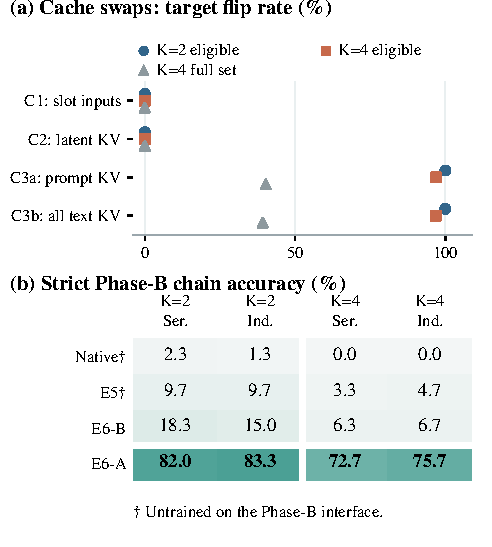
\includegraphics[width=\linewidth]{figs/fig3_e6c_double_dissociation.pdf}
  \caption{\textbf{Cache-Level Double Dissociation (\texttt{E6-C}) and Strict Phase-B In-Domain Accuracy (\texttt{E6-2} \& \texttt{E7-3b}).} \textbf{(a)} Under \texttt{E5} \texttt{Vision-Masked} decoding, swapping 28-layer $\KV_H$ caches yields $0.0\%$ flips, whereas swapping prefill $\KV_{Q,M}$ caches flips $96.9\%$--$100.0\%$ of eligible pairs ($40.2\%$ full set). \textbf{(b)} Under strict image-free Phase B on the 150 frozen clusters, step-aligned sub-windows (\texttt{E6-A}) achieve $72.7\%$--$83.3\%$ chain accuracy ($+63.7$ to $+69.0$pp over shared-prototype \texttt{E6-B}), driven synergistically by spatial ROI-MSE and color supervision.}
  \label{fig:e6c}
\end{figure}

\begin{figure*}[!t]
  \centering
  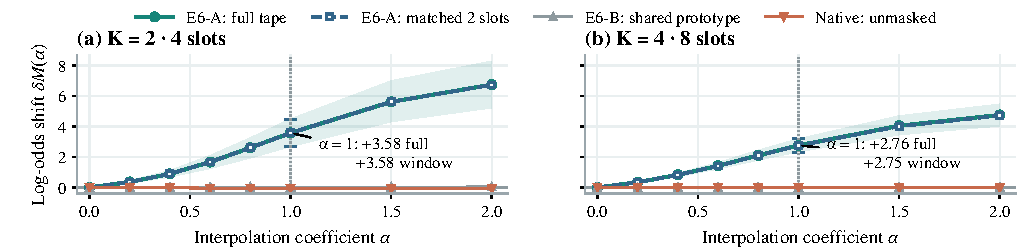
\includegraphics[width=\textwidth]{figs/fig4_e6_logit_interpolation.pdf}
  \caption{\textbf{Conditional Interpolation Logit Shift $\delta M(\alpha)$ Across All 266 Counterfactual Pairs (\texttt{E6-4e} vs.\ \texttt{E3-B2}).} Native \texttt{LVR-7B} and shared-prototype \texttt{E6-B} remain flat near zero, whereas \texttt{E6-A} drives a monotonic positive conditional log-odds shift ($+3.58$ on $K=2$, $+2.76$ on $K=4$ at $\alpha=1$). Interpolating \emph{only the 2 slots of the edited step} (dashed navy) matches the full-tape shift on the edited step ($+3.58$ on $K=2$, $+2.75$ on $K=4$). Both panels share the same vertical scale; shading shows full-tape $95\%$ cluster-bootstrap intervals and error bars at $\alpha=1$ show matched-window intervals.}
  \label{fig:logit_curves}
\end{figure*}

\textbf{28-Layer KV Double Dissociation (\texttt{E6-C}).} Because zeroing input vectors $H_{1:L} \leftarrow 0$ does not stop slot positions from attending to $\VT$ across layers (Proposition~\ref{prop:bypass}), we run four cache-level arms on \texttt{E5} under unified post-$\Mend$ \texttt{Vision-Masked} readout (\cref{tab:e6c} and \cref{fig:e6c}a): swapping all 28 layers of $\KV_H$ (\texttt{Arm C2}) yields \textbf{$0.00\%$} flips, whereas holding $\KV_H(\Vorig)$ fixed and swapping prefill caches $\KV_{Q,\mathrm{start}}(\Vrel)$ (\texttt{Arm C3a}) or $\KV_{Q,\mathrm{mkr}}(\Vrel)$ (\texttt{Arm C3b}) flips \textbf{$100.00\%$} of $K=2$ and $K=4$ chain-eligible pairs ($96.88\%$ position-eligible; $16.46\%$ and $39.19\%$--$40.23\%$ full set, matching the $16.46\%$ and $39.58\%$ all-visible donor reference). Feeding a black image to prefill $\KV_{Q,M}$ while keeping the real image's 28-layer $\KV_H(\VT)$ (\texttt{Arm C4}) drops \texttt{Vision-Masked} accuracy on the $150$ clusters by $\mathbf{64.00}$\textbf{pp to }$\mathbf{73.00}$\textbf{pp} ($69.67\% \to 3.33\%$ on $K=4$ serial), confirming that decoding-masked adaptation routes visual answers predominantly via $\KV_{Q,M}$.

\subsection{Strict Phase-B Readout, In-Vocab Control, Prior Trade-Offs, and Pointer Chaining (\texttt{E6} \& \texttt{E7})}
\label{subsec:exp_e6ab}

\textbf{In-Domain Accuracy and Supervision Ablation (\texttt{E6-2}, \texttt{E7-3b}).} Under Strict Phase B ($4$ epochs, $320$ updates on the $40$ dev clusters, checkpoints selected by 10-scene dev Phase-B answer CE; \cref{tab:e6_acc} and \cref{fig:e6c}b), untrained transfer of native \texttt{LVR-7B} ($0.00\%$--$2.33\%$) and \texttt{E5} ($3.33\%$--$9.67\%$) fails, and shared-prototype \texttt{E6-B} stalls at $15.00\%$--$18.33\%$ ($K=2$) and $6.33\%$--$6.67\%$ ($K=4$). In contrast, \textbf{\texttt{E6-A} achieves $82.00\%$--$83.33\%$ ($K=2$) and $72.67\%$--$75.67\%$ ($K=4$)}, outperforming \texttt{E6-B} by $\mathbf{+63.67}$\textbf{pp to }$\mathbf{+69.00}$\textbf{pp}. Ablating Phase-A supervision (\texttt{E7-3b}, \cref{tab:e6_acc} and Supplementary Table~S16) shows that \texttt{Answer-CE Only} collapses $K=4$ accuracy to $5.00\%$--$5.67\%$, whereas retaining only spatial alignment (\texttt{w/o Color-CE}: $73.67\%$--$77.33\%$ on $K=2$, $38.33\%$--$41.00\%$ on $K=4$) or only color supervision (\texttt{w/o ROI-MSE}: $80.00\%$--$81.67\%$ on $K=2$, $55.33\%$--$57.33\%$ on $K=4$) each beats \texttt{E6-B} and combines synergistically in \texttt{E6-A}.

\begin{table}[!t]
  \caption{\textbf{Strict Image-Free Phase-B Multi-Step Accuracy and Supervision/Prior Ablations on the 150 Frozen Clusters (\texttt{E6-2a} \& \texttt{E7-3b/1b}, $300$ Queries/Cond.).} Visual tokens $\VT$ and Phase-A KV caches are absent in Phase B. ($^\dagger$Zero-shot interface-transfer controls.)}
  \label{tab:e6_acc}
  \centering
  \resizebox{\linewidth}{!}{%
  \begin{tabular}{l c c c c c}
    \toprule
    & \multicolumn{2}{c}{\textbf{$K=2$ Chain (\%)}} & \multicolumn{2}{c}{\textbf{$K=4$ Chain / Pos (\%)}} & \textbf{vs.\ \texttt{E6-B}} \\
    \cmidrule(lr){2-3} \cmidrule(lr){4-5}
    \textbf{Model (Strict Phase B)} & \textbf{Serial} & \textbf{Indep.} & \textbf{Serial} & \textbf{Indep.} & \textbf{($K{=}4$ S/I, pp)} \\
    \midrule
    Native \texttt{LVR-7B}$^\dagger$ & $2.33$ & $1.33$ & $0.00 / 13.9$ & $0.00 / 13.0$ & — \\
    \texttt{E5} (Decode Mask)$^\dagger$ & $9.67$ & $9.67$ & $3.33 / 30.8$ & $4.67 / 32.2$ & — \\
    \texttt{E6-B} (Shared Proto) & $18.33$ & $15.00$ & $6.33 / 31.7$ & $6.67 / 31.2$ & Ref. \\
    \midrule
    \texttt{E7-3b} (\texttt{Answer-CE Only}) & $17.33$ & $16.00$ & $5.00 / 32.3$ & $5.67 / 31.8$ & $-1.3 / {-1.0}$ \\
    \texttt{E7-3b} (\texttt{w/o Color-CE}) & $73.67$ & $77.33$ & $38.33 / 70.0$ & $41.00 / 71.3$ & $+32.0 / +34.3$ \\
    \texttt{E7-3b} (\texttt{w/o ROI-MSE}) & $80.00$ & $81.67$ & $55.33 / 78.9$ & $57.33 / 79.0$ & $+49.0 / +50.7$ \\
    \texttt{E7-1b} (\texttt{8-Color + KL}) & $50.67$ & $53.33$ & $20.67 / 69.1$ & $18.00 / 69.2$ & $+14.3 / +11.3$ \\
    \rowcolor{resulttint}
    \textbf{\texttt{E6-A} (Full Step Win.)} & $\mathbf{82.00}$ & $\mathbf{83.33}$ & $\mathbf{72.67} / \mathbf{90.3}$ & $\mathbf{75.67} / \mathbf{91.3}$ & $\mathbf{+66.3 / +69.0}$ \\
    \bottomrule
  \end{tabular}%
  }
\end{table}

\begin{table}[!t]
  \caption{\textbf{Counterfactual Dissection on Unseen-Color ($266$ Pairs: \texttt{Yellow/Brown}) and In-Vocabulary ($496$ Pairs: \texttt{Red/Green/Blue}) Edits (\texttt{E6-3/4} \& \texttt{E7-1}).} Cells report $K{=}2 \;|\; K{=}4$ ($\%$, or pp for \texttt{Match$-$Unm}). Native/\texttt{E5} use 1-Stage \texttt{C1}; \texttt{E6/E7} rows use Strict Phase B.}
  \label{tab:e6_subwin}
  \centering
  \resizebox{\linewidth}{!}{%
  \begin{tabular}{l l c c c c}
    \toprule
    \textbf{Model / Edit Domain} & \textbf{Subset} & \textbf{Direct New} & \textbf{Orig$\to$New} & \textbf{Win Match / Unm} & \textbf{Match$-$Unm} \\
    ($K{=}2 \;|\; K{=}4$ Rec:Cl) & \textbf{Type} & ($K{=}2 \;|\; K{=}4$ \%) & ($K{=}2 \;|\; K{=}4$ \%) & ($K{=}2 \;|\; K{=}4$ \%) & ($K{=}2 \;|\; K{=}4$ pp) \\
    \midrule
    \multicolumn{6}{l}{\emph{Part A: Held-Out Unseen Colors (\texttt{Yellow/Brown}, $92{:}41 \;|\; 174{:}64$ Full Set)}} \\
    Nat.\ / \texttt{E5} (1-Stg \texttt{C1}) & Full & $68.9/16.5 \;|\; 59.2/41.1$ & $1.2/0.0 \;|\; 0.3/0.0$ & $\text{—} \;|\; \text{—}$ & $\text{—} \;|\; \text{—}$ \\
    \texttt{E6-B} (Shared Proto) & Full & $0.0 \;|\; 0.0$ & $0.0 \;|\; 0.0$ & $0.0/0.0 \;|\; 0.0/0.0$ & $0.0 \;|\; 0.0$ \\
    \texttt{E6-A} (Unseen Raw) & Full & $0.0 \;|\; 3.1$ & $0.0 \;|\; 3.1$ & $0.0/0.0 \;|\; 3.1/0.0$ & $0.0 \;|\; +3.1$ \\
    \texttt{E6-A} (Unseen Raw) & Elig ($0|5{:}4$) & $\text{NA} \;|\; 100$ & $\text{NA} \;|\; 100$ & $\text{NA} \;|\; 100/0.0$ & $\text{NA} \;|\; +100$ \\
    \texttt{E7-1a-P} (Prior Calib.) & Full & $23.8 \;|\; 45.2$ & $18.9 \;|\; 35.4$ & $\text{—} \;|\; \text{—}$ & $\text{—} \;|\; \text{—}$ \\
    \rowcolor{resulttint}
    \textbf{\texttt{E7-1b} (\texttt{8-Color+KL})} & Full & $\mathbf{85.4} \;|\; \mathbf{82.3}$ & $\mathbf{57.3} \;|\; \mathbf{47.8}$ & $\mathbf{85.4}/25.6 \;|\; \mathbf{81.5}/34.5$ & $\mathbf{+59.8} \;|\; \mathbf{+47.1}$ \\
    \rowcolor{resulttint}
    \textbf{\texttt{E7-1b} (\texttt{8-Color+KL})} & Elig ($50{:}26|84{:}37$) & $\mathbf{100} \;|\; \mathbf{100}$ & $\mathbf{100} \;|\; \mathbf{100}$ & $\mathbf{100}/0.0 \;|\; \mathbf{98.7}/0.7$ & $\mathbf{+100} \;|\; \mathbf{+98.0}$ \\
    \midrule
    \multicolumn{6}{l}{\emph{Part B: In-Vocabulary Seen Colors (\texttt{Red $\leftrightarrow$ Green $\leftrightarrow$ Blue}, $176{:}39 \;|\; 320{:}62$ Full Set, \texttt{E7-1a})}} \\
    \texttt{E6-B} (In-Vocab) & Full & $29.8 \;|\; 33.7$ & $0.0 \;|\; 1.6$ & $29.5/29.5 \;|\; 34.8/33.6$ & $0.0 \;|\; +1.3$ \\
    \rowcolor{resulttint}
    \textbf{\texttt{E6-A} (In-Vocab)} & Full & $\mathbf{73.4} \;|\; \mathbf{58.5}$ & $\text{—}$ & $\mathbf{73.4}/3.2 \;|\; \mathbf{59.5}/1.5$ & $\mathbf{+70.2} \;|\; \mathbf{+58.1}$ \\
    \rowcolor{resulttint}
    \textbf{\texttt{E6-A} (In-Vocab)} & Elig ($121{:}36|187{:}49$) & $\mathbf{100} \;|\; \mathbf{100}$ & $\mathbf{100} \;|\; \mathbf{100}$ & $\mathbf{100}/0.0 \;|\; \mathbf{99.2}/0.2$ & $\mathbf{+100} \;|\; \mathbf{+99.0}$ \\
    \bottomrule
  \end{tabular}%
  }
\end{table}

\textbf{In-Vocabulary Local Control vs.\ Unseen-Color Prior Trade-Offs (\texttt{E6-3/4}, \texttt{E7-1}, \texttt{E7-3a}).} Comparing unseen-color and in-vocabulary edits (\cref{tab:e6_subwin}, \cref{fig:logit_curves}, Supplementary Tables~S13, S15, S16) isolates sub-window control from priors:
(1) \emph{Seen-Color Control (\texttt{E7-1a}):} Rotating within seen colors (\texttt{red/green/blue}, $496$ records / $62$ clusters), \texttt{E6-A} achieves \textbf{$73.40\%/58.53\%$ ($K{=}2/4$) full-set flips}, with \texttt{Win-Matched} vs.\ \texttt{Win-Unmatched} rates of $\mathbf{73.40\%}$ \textbf{vs.\ }$\mathbf{3.21\%}$ ($\mathbf{+70.19}$\textbf{pp}) on $K=2$ and $\mathbf{59.54\%}$ \textbf{vs.\ }$\mathbf{1.48\%}$ ($\mathbf{+58.06}$\textbf{pp}) on $K=4$ ($+70.19/+56.81$pp DID over \texttt{E6-B}; $\mathbf{100.00}/\mathbf{99.03}$\textbf{pp} on eligible subsets of $121/36$ and $187/49$).
(2) \emph{Full $K\times K$ Matrix (\texttt{E7-3a}):} Probing all $K\times K$ shifts $\delta M_{k \leftarrow r}(1)$ (Supplementary Table~S15) shows diagonal dominance ($\delta M_{r \leftarrow r}(1) \in [+0.21, +3.44]$ log-odds) alongside forward spillover to $k = r+1$ ($+0.376$ on $K=2$; $+0.154$ to $+0.209$ on $K=4$), with cluster-mean max off-diagonal shift of $0.486\ci{0.337}{0.646}$ ($K=2$) and $0.697\ci{0.562}{0.847}$ ($K=4$).
(3) \emph{Unseen-Color Trade-Offs (\texttt{E7-1a-P}, \texttt{E7-1b}):} On held-out \texttt{yellow/brown} ($266$ pairs), 3-color priors limit raw \texttt{E6-A} flips to $0.00\%/3.12\%$ ($K{=}2/4$; $5$ eligible records / $4$ clusters), despite $+3.58/+2.75$ matched-window shifts and $80.49$--$81.25$pp slot-zeroing drops on $\Vorig$. Subtracting zero-slot shifts (\texttt{E7-1a-P}) lifts free flips to $23.78\%/45.18\%$ ($18.90\%/35.42\%$ joint $\Vorig\text{-correct}\to\text{new}$) at a $-7.32/{-34.38}\text{pp}$ $\Vorig$ accuracy cost. Likewise, \texttt{8-Color + KL} (\texttt{E7-1b}) reaches $\mathbf{85.37\%/82.29\%}$ new-color rate ($57.32\%/47.79\%$ joint flips, $+59.76/+47.05$pp \texttt{Matched$-$Unmatched}), but shows $25.61\%/34.46\%$ unmatched spillover and drops 150-scene \texttt{E1} $K=4$ accuracy to $20.67\%/18.00\%$ (\cref{tab:e6_acc}).

\textbf{Implicit Pointer Chaining (\texttt{E7-4}).} On the $600$ pointer-chaining queries (Supplementary Table~S17), 4-epoch ($160$-update) Strict Phase-B training shows that \textbf{Recurrent Phase-A beats Parallel Phase-A by $\mathbf{+10.00}\ci{3.00}{17.00}$\textbf{pp} on $K=2$ ($80.67\%$ vs.\ $70.67\%$) and $\mathbf{+10.00}\ci{1.33}{18.67}$\textbf{pp} on $K=4$ ($41.33\%$ vs.\ $31.33\%$)} ($+8.67/+10.67$pp on final step $O_K$). However, same-weight direct vision (\texttt{NoLatent}) reaches $85.00\%/59.33\%$ (Parallel) and $87.33\%/63.00\%$ (Recurrent), exceeding Strict Phase B by $6.67$--$28.00$pp (DID $+7.67/+6.33$pp). Thus recurrent emission narrows isolation loss without surpassing direct vision.
